\documentclass[xcolor={x11names}, aspectratio=169]{beamer}

\usepackage{tikz}
\usepackage{pgfplots}
\pgfplotsset{compat=1.18}

\usepackage{amsmath,amssymb,amsthm}
\usepackage{mathtools}
\usepackage{tcolorbox}
\usepackage{booktabs}
\usepackage{multirow}
\usepackage{colortbl}
\usepackage{array}

\usetikzlibrary{arrows.meta, positioning, patterns, calc, shapes, shapes.geometric, decorations.pathreplacing, quotes, backgrounds, fit, intersections}

% Theme settings
\usetheme{Madrid}
\usecolortheme{whale}
\setbeamertemplate{navigation symbols}{}

% Custom colors
\definecolor{navyblue}{RGB}{0,32,63}
\definecolor{goldaccent}{RGB}{197,164,103}
\definecolor{steelgray}{RGB}{70,84,98}
\definecolor{lightgray}{RGB}{245,245,247}
\definecolor{formulabg}{RGB}{250,248,245}

\setbeamercolor{palette primary}{bg=navyblue,fg=white}
\setbeamercolor{palette secondary}{bg=steelgray,fg=white}
\setbeamercolor{palette tertiary}{bg=goldaccent,fg=navyblue}
\setbeamercolor{structure}{fg=navyblue}
\setbeamercolor{title}{fg=navyblue}
\setbeamercolor{frametitle}{fg=navyblue,bg=lightgray}

% Navigation headline
\setbeamertemplate{headline}{%
  \leavevmode%
  \hbox{%
    \begin{beamercolorbox}[wd=\paperwidth,ht=2.5ex,dp=1.125ex]{palette primary}%
      \insertsectionnavigationhorizontal{\paperwidth}{}{\hskip0pt plus1filll}
    \end{beamercolorbox}%
  }
}

% Footline
\setbeamertemplate{footline}{%
  \leavevmode%
  \hbox{%
    \begin{beamercolorbox}[wd=.333333\paperwidth,ht=2.25ex,dp=1ex,center]{palette primary}%
      \usebeamerfont{author in head/foot}\insertshortauthor
    \end{beamercolorbox}%
    \begin{beamercolorbox}[wd=.333333\paperwidth,ht=2.25ex,dp=1ex,center]{palette secondary}%
      \usebeamerfont{title in head/foot}\insertshorttitle
    \end{beamercolorbox}%
    \begin{beamercolorbox}[wd=.333333\paperwidth,ht=2.25ex,dp=1ex,right]{palette primary}%
      \insertframenumber{} / \inserttotalframenumber\hspace*{2ex}
    \end{beamercolorbox}%
  }%
}

% Custom commands
\newcommand{\E}{\mathbb{E}}
\newcommand{\Var}{\text{Var}}
\newcommand{\Cov}{\text{Cov}}
\newcommand{\pmark}{\partial}

% Compact boxes
\newtcolorbox{formulabox}[1][]{
    colback=formulabg, colframe=goldaccent, boxrule=1.5pt, arc=2pt,
    left=6pt, right=6pt, top=4pt, bottom=4pt,
    fonttitle=\bfseries\small\color{navyblue}, title={#1}
}
\newtcolorbox{defbox}[1][]{
    colback=lightgray, colframe=navyblue, boxrule=1pt, arc=2pt,
    left=6pt, right=6pt, top=4pt, bottom=4pt,
    fonttitle=\bfseries\small, title={#1}
}
\newtcolorbox{prosbox}{
    colback=green!5, colframe=green!50!black, boxrule=1pt, arc=2pt,
    left=4pt, right=4pt, top=3pt, bottom=3pt
}
\newtcolorbox{consbox}{
    colback=red!5, colframe=red!50!black, boxrule=1pt, arc=2pt,
    left=4pt, right=4pt, top=3pt, bottom=3pt
}

\newcommand{\sectionslide}{%
  \begin{frame}
    \vfill
    \centering
    \begin{beamercolorbox}[sep=10pt,center,shadow=true,rounded=true]{palette primary}
      \usebeamerfont{title}\Large\insertsectionhead\par%
    \end{beamercolorbox}
    \vfill
  \end{frame}
}

\newcommand{\partslide}{%
  \begin{frame}
    \vfill
    \centering
    \begin{beamercolorbox}[sep=14pt,center,shadow=true,rounded=true]{palette primary}
      \usebeamerfont{title}\LARGE\insertpart\par%
    \end{beamercolorbox}
    \vfill
  \end{frame}
}

\title{Mortgage-Backed Security Hedging}
\subtitle{Risk Metrics, Instruments, and Mathematical Foundations}
\author{Quantitative Finance Series}
\date{\today}

\begin{document}

\begin{frame}
  \titlepage
\end{frame}

\begin{frame}{Roadmap}
  \tableofcontents[hideallsubsections]
\end{frame}

%===============================================
\part{Foundations}
\partslide
\section{The MBS Hedging Challenge}
%===============================================

\begin{frame}{Why Hedge Mortgage-Backed Securities?}
\textbf{The Fundamental Problem:} MBS have complex interest rate sensitivity

\begin{center}
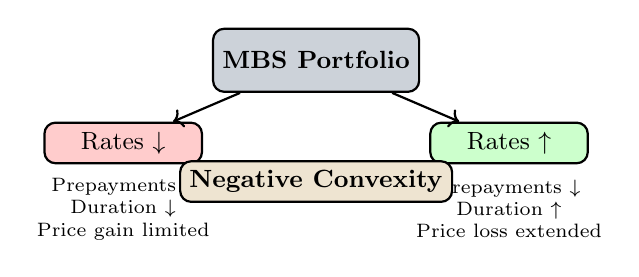
\begin{tikzpicture}[scale=0.7]
  \node[draw, thick, fill=navyblue!20, rounded corners, minimum width=2.5cm, minimum height=0.8cm] (mbs) at (0,0) {\small\textbf{MBS Portfolio}};
  
  \node[draw, thick, fill=red!20, rounded corners, minimum width=2cm] (down) at (-3.5,-1.5) {\small Rates $\downarrow$};
  \node[draw, thick, fill=green!20, rounded corners, minimum width=2cm] (up) at (3.5,-1.5) {\small Rates $\uparrow$};
  
  \node[align=center, font=\scriptsize] at (-3.5,-2.7) {Prepayments $\uparrow$\\Duration $\downarrow$\\Price gain limited};
  \node[align=center, font=\scriptsize] at (3.5,-2.7) {Prepayments $\downarrow$\\Duration $\uparrow$\\Price loss extended};
  
  \draw[->, thick] (mbs) -- (down);
  \draw[->, thick] (mbs) -- (up);
  
  \node[draw, thick, fill=goldaccent!30, rounded corners] at (0,-2.2) {\small\textbf{Negative Convexity}};
\end{tikzpicture}
\end{center}

\textbf{Key Risks:} Interest rate risk, prepayment risk, basis risk, volatility risk.
\end{frame}

\begin{frame}{The Prepayment Option: Mathematical View}
\begin{defbox}[Embedded Option Structure]
The MBS holder has \textbf{sold} a call option to the borrower: $V_{MBS} = V_{bond} - V_{call}$
\end{defbox}

\textbf{Option Characteristics:} Strike = principal balance, American-style exercise, moneyness determined by current rate vs.\ coupon.

\textbf{Impact on Price-Yield Relationship:}
\[
\frac{\pmark P}{\pmark y} < 0 \quad \text{(always)} \qquad \frac{\pmark^2 P}{\pmark y^2} < 0 \quad \text{(negative convexity when ITM)}
\]

The \textbf{gamma} of the embedded short call creates the hedging challenge.
\end{frame}

\begin{frame}{The Hedging Universe: Instrument Overview}
\begin{center}
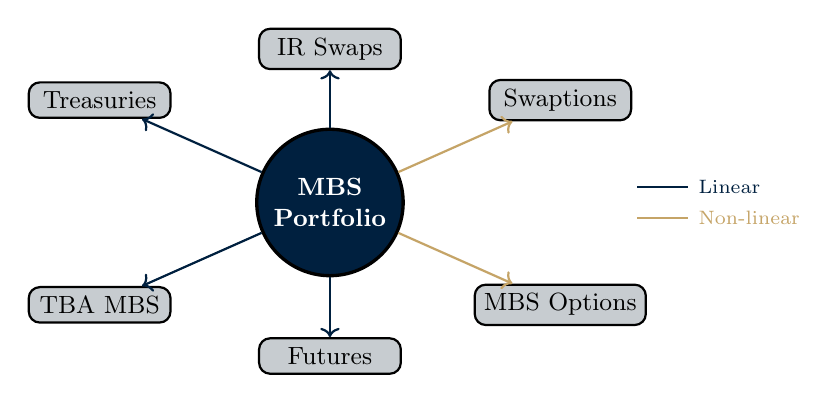
\begin{tikzpicture}[scale=0.65]
  \node[draw, very thick, fill=navyblue, text=white, circle, minimum size=1.8cm, align=center, font=\small] (center) at (0,0) {\textbf{MBS}\\\textbf{Portfolio}};
  
  \node[draw, thick, fill=steelgray!30, rounded corners, minimum width=1.8cm, font=\small] (tsy) at (-4.5,2) {Treasuries};
  \node[draw, thick, fill=steelgray!30, rounded corners, minimum width=1.8cm, font=\small] (swaps) at (0,3) {IR Swaps};
  \node[draw, thick, fill=steelgray!30, rounded corners, minimum width=1.8cm, font=\small] (swaptions) at (4.5,2) {Swaptions};
  \node[draw, thick, fill=steelgray!30, rounded corners, minimum width=1.8cm, font=\small] (tba) at (-4.5,-2) {TBA MBS};
  \node[draw, thick, fill=steelgray!30, rounded corners, minimum width=1.8cm, font=\small] (futures) at (0,-3) {Futures};
  \node[draw, thick, fill=steelgray!30, rounded corners, minimum width=1.8cm, font=\small] (options) at (4.5,-2) {MBS Options};
  
  \draw[->, thick, navyblue] (center) -- (tsy);
  \draw[->, thick, navyblue] (center) -- (swaps);
  \draw[->, thick, goldaccent] (center) -- (swaptions);
  \draw[->, thick, navyblue] (center) -- (tba);
  \draw[->, thick, navyblue] (center) -- (futures);
  \draw[->, thick, goldaccent] (center) -- (options);
  
  \draw[thick, navyblue] (6,0.3) -- (7,0.3) node[right, font=\scriptsize] {Linear};
  \draw[thick, goldaccent] (6,-0.3) -- (7,-0.3) node[right, font=\scriptsize] {Non-linear};
\end{tikzpicture}
\end{center}
\end{frame}

%===============================================
\section{Core Risk Metrics}
\sectionslide
%===============================================

\begin{frame}{Dollar Value of a Basis Point (DV01)}
\begin{defbox}[Definition: DV01]
\textbf{DV01} measures the dollar change in value for a 1 bp change in yield:
$\boxed{DV01 = -\frac{\pmark P}{\pmark y} \times 0.0001}$
\end{defbox}

\textbf{Mathematical Derivation:}
For price $P(y)$: $\Delta P \approx \frac{\pmark P}{\pmark y} \Delta y$. Setting $\Delta y = 0.0001$:
\[
DV01 = -\Delta P = -\frac{\pmark P}{\pmark y} \times 0.0001
\]

\textbf{For a coupon bond:} $\displaystyle DV01 = \frac{1}{10000} \sum_{i=1}^{n} t_i \cdot C_{t_i} e^{-y \cdot t_i}$
\end{frame}

\begin{frame}{Duration: The First-Order Sensitivity}
\begin{defbox}[Duration Definitions]
\textbf{Macaulay:} $D_{mac} = \frac{\sum_{i} t_i \cdot PV(C_{t_i})}{P}$ \quad
\textbf{Modified:} $D_{mod} = \frac{D_{mac}}{1 + y/k} = -\frac{1}{P} \frac{\pmark P}{\pmark y}$
\end{defbox}

\textbf{Effective Duration (for MBS):}
\[
\boxed{D_{eff} = -\frac{P_{-\Delta y} - P_{+\Delta y}}{2 \cdot P_0 \cdot \Delta y}}
\]

\textbf{Key Relationships:}
\[
\frac{\Delta P}{P} \approx -D_{mod} \cdot \Delta y \qquad DV01 = \frac{D_{mod} \times P}{10000}
\]
\end{frame}

\begin{frame}{Convexity: The Second-Order Effect}
\begin{defbox}[Convexity Definition]
\textbf{Convexity} measures curvature: $\boxed{C = \frac{1}{P} \frac{\pmark^2 P}{\pmark y^2}}$
\end{defbox}

\textbf{Taylor Expansion:} $\displaystyle\frac{\Delta P}{P} \approx -D_{mod} \cdot \Delta y + \frac{1}{2} C \cdot (\Delta y)^2$

\textbf{Effective Convexity:} $\boxed{C_{eff} = \frac{P_{-\Delta y} + P_{+\Delta y} - 2P_0}{P_0 \cdot (\Delta y)^2}}$

\textbf{MBS Convexity:} Positive when rates high (OTM), \textbf{negative} when rates low (ITM).
\end{frame}

\begin{frame}{Visualizing Duration and Convexity}
\begin{center}
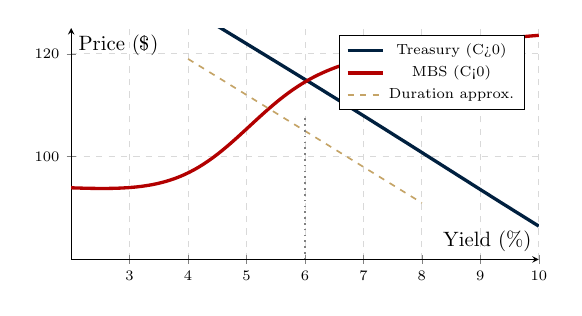
\begin{tikzpicture}[scale=0.75]
  \begin{axis}[
    xlabel={Yield (\%)}, ylabel={Price (\$)},
    xmin=2, xmax=10, ymin=80, ymax=125,
    axis lines=middle, width=9.5cm, height=5.5cm,
    grid=major, grid style={dashed, gray!30},
    tick label style={font=\scriptsize},
    legend pos=north east, legend style={font=\scriptsize}
  ]
  
  \addplot[domain=2:10, samples=100, ultra thick, navyblue] {100*exp(-0.07*(x-6)) + 15*exp(-0.02*(x-6)^2)};
  \addlegendentry{Treasury (C>0)}
  
  \addplot[domain=2:10, samples=100, ultra thick, red!70!black] {95 + 30/(1+exp(-1.5*(x-5))) - 5*exp(-0.08*(x-6)^2)};
  \addlegendentry{MBS (C<0)}
  
  \addplot[domain=4:8, samples=2, thick, dashed, goldaccent] {105 - 7*(x-6)};
  \addlegendentry{Duration approx.}
  
  \draw[thick, dotted, gray] (axis cs:6,80) -- (axis cs:6,108);
  \end{axis}
\end{tikzpicture}
\end{center}
\end{frame}

\begin{frame}{Key Rate Duration (KRD)}
\begin{defbox}[Key Rate Duration]
\textbf{KRD} = sensitivity to shifts at specific curve points: $KRD_i = -\frac{1}{P} \frac{\pmark P}{\pmark y_i}$
\end{defbox}

\textbf{Decomposition:} $D_{eff} = \sum_{i=1}^{n} KRD_i$

\begin{center}
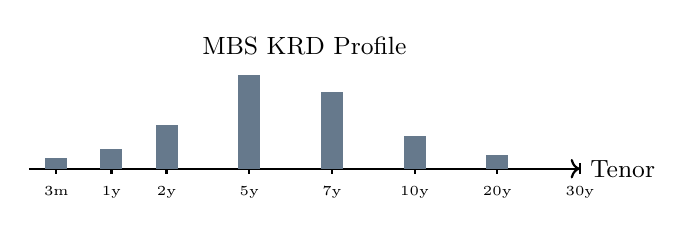
\begin{tikzpicture}[scale=0.7]
  \draw[thick, ->] (0,0) -- (10,0) node[right] {\small Tenor};
  \foreach \x/\label in {0.5/3m, 1.5/1y, 2.5/2y, 4/5y, 5.5/7y, 7/10y, 8.5/20y, 10/30y} {
    \draw[thick] (\x,0.1) -- (\x,-0.1);
    \node[below, font=\tiny] at (\x,-0.15) {\label};
  }
  
  \fill[navyblue!60] (0.3,0) rectangle (0.7,0.2);
  \fill[navyblue!60] (1.3,0) rectangle (1.7,0.35);
  \fill[navyblue!60] (2.3,0) rectangle (2.7,0.8);
  \fill[navyblue!60] (3.8,0) rectangle (4.2,1.7);
  \fill[navyblue!60] (5.3,0) rectangle (5.7,1.4);
  \fill[navyblue!60] (6.8,0) rectangle (7.2,0.6);
  \fill[navyblue!60] (8.3,0) rectangle (8.7,0.25);
  
  \node[above, font=\small] at (5,1.9) {MBS KRD Profile};
\end{tikzpicture}
\end{center}
\end{frame}

%===============================================
\section{Extended Greeks}
\sectionslide
%===============================================

\begin{frame}{Vega: Volatility Sensitivity}
\begin{defbox}[Option-Adjusted Vega (OAV)]
\textbf{Vega} measures price sensitivity to implied volatility:
$\boxed{\text{Vega} = \frac{\pmark P}{\pmark \sigma}}$
\end{defbox}

\textbf{For MBS:} Since MBS = Bond $-$ Call Option:
\[
\text{Vega}_{MBS} = -\text{Vega}_{call} < 0
\]

\textbf{Interpretation:} MBS prices \textit{fall} when volatility rises (short option position).

\textbf{Vega Hedge Ratio:}
\[
N_{swaption} = -\frac{\text{Vega}_{MBS}}{\text{Vega}_{swaption}}
\]
\end{frame}

\begin{frame}{Theta: Time Decay}
\begin{defbox}[Time Decay]
\textbf{Theta} measures value change with passage of time:
$\boxed{\Theta = \frac{\pmark P}{\pmark t}}$
\end{defbox}

\textbf{For Hedged MBS Positions:}
\[
\Theta_{portfolio} = \Theta_{MBS} + \Theta_{hedge}
\]

\textbf{Key Insight:} Swaption hedges have negative theta (time decay cost):
\begin{itemize}
  \item Long straddle: $\Theta < 0$ (pays for convexity protection)
  \item Must balance theta cost against convexity benefit
\end{itemize}

\textbf{Carry vs.\ Roll-down:} Total return = Coupon $+$ Roll-down $+$ Theta
\end{frame}

\begin{frame}{Cross-Gamma: Rate-Volatility Interaction}
\begin{defbox}[Cross-Gamma]
\textbf{Cross-gamma} measures how delta changes with volatility:
$\boxed{\Gamma_{r,\sigma} = \frac{\pmark^2 P}{\pmark r \, \pmark \sigma} = \frac{\pmark \Delta}{\pmark \sigma} = \frac{\pmark \text{Vega}}{\pmark r}}$
\end{defbox}

\textbf{Implication for MBS:}
\begin{itemize}
  \item Duration changes when volatility changes
  \item Vega changes when rates change
  \item Creates ``correlation risk'' in hedges
\end{itemize}

\textbf{Practical Impact:}
\[
\Delta P \approx -D \cdot \Delta r + \text{Vega} \cdot \Delta\sigma + \Gamma_{r,\sigma} \cdot \Delta r \cdot \Delta\sigma
\]

In volatile markets, cross-gamma can dominate P\&L.
\end{frame}

\begin{frame}{Complete Greeks Summary}
\begin{center}
\renewcommand{\arraystretch}{1.15}
\small
\begin{tabular}{l|c|c|c}
\toprule
\textbf{Greek} & \textbf{Formula} & \textbf{MBS Sign} & \textbf{Hedge With} \\
\midrule
\rowcolor{navyblue!10}
Delta ($\Delta$) & $\frac{\pmark P}{\pmark r}$ & Negative & Swaps, Treasuries \\
Gamma ($\Gamma$) & $\frac{\pmark^2 P}{\pmark r^2}$ & Negative (low rates) & Swaptions \\
\rowcolor{navyblue!10}
Vega ($\mathcal{V}$) & $\frac{\pmark P}{\pmark \sigma}$ & Negative & Swaptions \\
Theta ($\Theta$) & $\frac{\pmark P}{\pmark t}$ & Positive (carry) & -- \\
\rowcolor{navyblue!10}
Cross-$\Gamma$ & $\frac{\pmark^2 P}{\pmark r \pmark \sigma}$ & Variable & Complex structures \\
\bottomrule
\end{tabular}
\end{center}

\textbf{Full P\&L Decomposition:}
\[
\Delta P = \Delta \cdot dr + \frac{1}{2}\Gamma \cdot dr^2 + \mathcal{V} \cdot d\sigma + \Theta \cdot dt + \Gamma_{r,\sigma} \cdot dr \cdot d\sigma
\]
\end{frame}

%===============================================
\part{Prepayment Modeling}
\partslide
\section{Prepayment Conventions}
%===============================================

\begin{frame}{CPR, SMM, and PSA Conventions}
\begin{defbox}[Prepayment Rate Definitions]
\textbf{CPR} (Conditional Prepayment Rate): Annualized prepayment rate
\[
CPR = 1 - \left(\frac{\text{Remaining Balance}}{\text{Scheduled Balance}}\right)^{12}
\]

\textbf{SMM} (Single Monthly Mortality): Monthly prepayment rate
\[
\boxed{SMM = 1 - (1 - CPR)^{1/12}}
\]
\end{defbox}

\textbf{PSA Benchmark:}
\[
CPR_t = \min\left(\frac{t}{30}, 1\right) \times 6\%
\]
where $t$ = loan age in months. 100\% PSA ramps from 0\% to 6\% CPR over 30 months.
\end{frame}

\begin{frame}{PSA Ramp Visualization}
\begin{center}
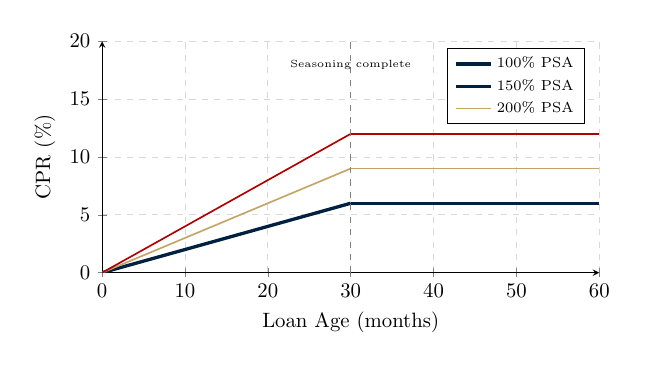
\begin{tikzpicture}[scale=0.75]
  \begin{axis}[
    xlabel={Loan Age (months)}, ylabel={CPR (\%)},
    xmin=0, xmax=60, ymin=0, ymax=20,
    axis lines=left, width=10cm, height=5.5cm,
    grid=major, grid style={dashed, gray!30},
    legend pos=north east, legend style={font=\scriptsize}
  ]
  
  % 100% PSA
  \addplot[domain=0:30, samples=31, ultra thick, navyblue] {0.2*x};
  \addplot[domain=30:60, samples=31, ultra thick, navyblue] {6};
  \addlegendentry{100\% PSA}
  
  % 150% PSA
  \addplot[domain=0:30, samples=31, thick, goldaccent] {0.3*x};
  \addplot[domain=30:60, samples=31, thick, goldaccent] {9};
  \addlegendentry{150\% PSA}
  
  % 200% PSA
  \addplot[domain=0:30, samples=31, thick, red!70!black] {0.4*x};
  \addplot[domain=30:60, samples=31, thick, red!70!black] {12};
  \addlegendentry{200\% PSA}
  
  \draw[dashed, gray] (axis cs:30,0) -- (axis cs:30,20);
  \node[font=\tiny] at (axis cs:30,18) {Seasoning complete};
  
  \end{axis}
\end{tikzpicture}
\end{center}
\end{frame}

\begin{frame}{The Prepayment S-Curve}
\begin{defbox}[Refinancing Incentive]
\textbf{Incentive} = WAC $-$ Current Rate. Prepayment: $CPR(x) = CPR_{min} + \frac{CPR_{max} - CPR_{min}}{1 + e^{-\beta(x - x_0)}}$
\end{defbox}
\vspace{-0.2cm}
\begin{center}
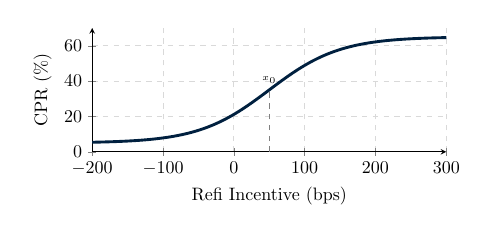
\begin{tikzpicture}[scale=0.65]
  \begin{axis}[
    xlabel={Refi Incentive (bps)}, ylabel={CPR (\%)},
    xmin=-200, xmax=300, ymin=0, ymax=70,
    axis lines=left, width=8.5cm, height=4cm,
    grid=major, grid style={dashed, gray!30}
  ]
  
  \addplot[domain=-200:300, samples=100, ultra thick, navyblue] {5 + 60/(1+exp(-0.02*(x-50)))};
  
  \draw[dashed, gray] (axis cs:50,0) -- (axis cs:50,35);
  \node[font=\tiny, above] at (axis cs:50,35) {$x_0$};
  
  \end{axis}
\end{tikzpicture}
\end{center}
\end{frame}

\begin{frame}{Burnout Effect: Path Dependency}
\begin{defbox}[Burnout Model]
\textbf{Burnout} = Reduction in prepayment response after sustained low rates

Cumulative refinancing opportunity:
\[
B_t = \int_0^t \max(0, \text{Incentive}_s) \, ds
\]

Adjusted CPR:
\[
\boxed{CPR_{adj} = CPR_{base} \times e^{-\lambda B_t}}
\]
where $\lambda$ = burnout decay rate.
\end{defbox}

\textbf{Intuition:} Borrowers most likely to refinance do so first; remaining pool is ``burned out.''
\end{frame}

\begin{frame}{Prepayment Components}
\begin{center}
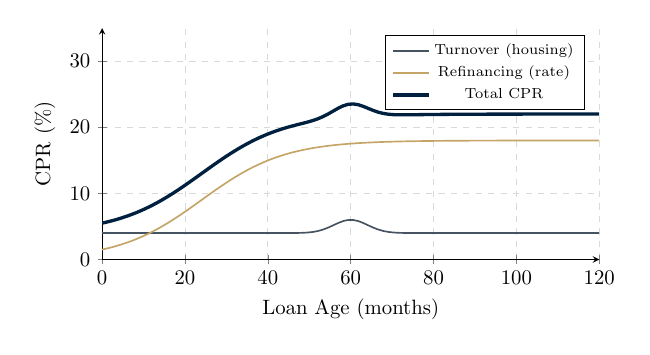
\begin{tikzpicture}[scale=0.75]
  \begin{axis}[
    xlabel={Loan Age (months)}, ylabel={CPR (\%)},
    xmin=0, xmax=120, ymin=0, ymax=35,
    axis lines=left, width=10cm, height=5.5cm,
    grid=major, grid style={dashed, gray!30},
    legend pos=north east, legend style={font=\scriptsize}
  ]
  
  % Turnover (baseline)
  \addplot[domain=0:120, samples=100, thick, steelgray] {4 + 2*exp(-0.03*(x-60)^2)};
  \addlegendentry{Turnover (housing)}
  
  % Refinancing
  \addplot[domain=0:120, samples=100, thick, goldaccent] {18/(1+exp(-0.1*(x-24)))};
  \addlegendentry{Refinancing (rate)}
  
  % Total
  \addplot[domain=0:120, samples=100, ultra thick, navyblue] {4 + 2*exp(-0.03*(x-60)^2) + 18/(1+exp(-0.1*(x-24)))};
  \addlegendentry{Total CPR}
  
  \end{axis}
\end{tikzpicture}
\end{center}

\textbf{Total CPR} = Turnover + Refinancing + Curtailments + Defaults
\end{frame}

%===============================================
\part{Hedging Instruments}
\partslide
\section{Linear Hedges}
%===============================================

\begin{frame}{Treasury Securities as Hedges}
\begin{columns}[T]
\begin{column}{0.48\textwidth}
\begin{prosbox}
\textbf{Advantages:}
\begin{itemize}\small
  \item Highest liquidity
  \item No credit risk
  \item Multiple maturities
  \item Simple execution
\end{itemize}
\end{prosbox}
\end{column}

\begin{column}{0.48\textwidth}
\begin{consbox}
\textbf{Disadvantages:}
\begin{itemize}\small
  \item Convexity mismatch
  \item Basis risk
  \item Cannot hedge spread
  \item Carry cost
\end{itemize}
\end{consbox}
\end{column}
\end{columns}

\vspace{0.2cm}
\begin{formulabox}[Treasury Hedge Ratio]
$HR_{TSY} = \frac{DV01_{MBS}}{DV01_{TSY}} = \frac{D_{MBS} \times P_{MBS}}{D_{TSY} \times P_{TSY}}$
\end{formulabox}
\end{frame}

\begin{frame}{Interest Rate Swap Hedging}
\begin{defbox}[Swap DV01]
$DV01_{swap} = DV01_{fixed} - DV01_{float} \approx DV01_{fixed}$ (floating resets to par)
\end{defbox}

\begin{formulabox}[Swap Hedge Ratio]
$\boxed{N_{swap} = -\frac{DV01_{MBS}}{DV01_{swap}} \times P_{MBS}}$
\end{formulabox}

\textbf{Example:} MBS with DV01 = \$43,050, 5Y swap DV01 = \$45/\$1M

$\Rightarrow$ Hedge notional $= \frac{\$43,050}{\$45/\text{M}} = \$95.7\text{M}$
\end{frame}

\begin{frame}{TBA and Dollar Roll}
\begin{defbox}[TBA = To-Be-Announced]
Forward contract on generic MBS pools. Natural hedge for MBS portfolios.
\end{defbox}

\textbf{Dollar Roll:} Sell near-month TBA, buy far-month TBA.
\[
\text{Roll Value} = P_{near} - P_{far} - \Delta\text{AI}
\]

\textbf{Implied Financing Rate:}
\[
r_{implied} = \frac{(P_{near} - P_{far}) \times 12/\text{days}}{P_{near}}
\]

\textbf{Advantage:} TBA has similar convexity profile to specified pools.
\end{frame}

%===============================================
\section{Non-Linear Hedges}
%===============================================

\begin{frame}{Swaptions: Hedging Negative Convexity}
\begin{defbox}[Swaption Greeks]
\textbf{Receiver Swaption:} $\Delta < 0$, $\Gamma > 0$, Vega $> 0$
\end{defbox}

\textbf{Straddle Strategy:} Buy receiver + payer at same strike
\[
\Gamma_{straddle} = \Gamma_{rcvr} + \Gamma_{payer} > 0
\]

\textbf{Hedge Ratios:}
\[
N_{\Gamma} = -\frac{C_{MBS} \times P_{MBS}}{\Gamma_{swaption}} \qquad N_{\mathcal{V}} = -\frac{\text{Vega}_{MBS}}{\text{Vega}_{swaption}}
\]

\textbf{Trade-off:} Convexity protection costs theta (time decay).
\end{frame}

\begin{frame}{Swaption Convexity Hedge: Visualization}
\begin{center}
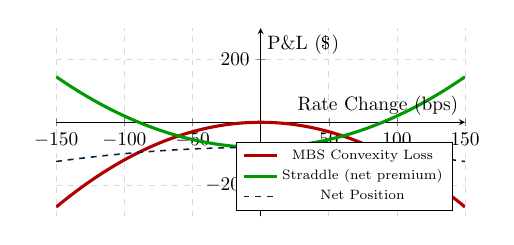
\begin{tikzpicture}[scale=0.7]
  \begin{axis}[
    xlabel={Rate Change (bps)}, ylabel={P\&L (\$)},
    xmin=-150, xmax=150, ymin=-300, ymax=300,
    axis lines=middle, width=9cm, height=5cm,
    grid=major, grid style={dashed, gray!30},
    legend pos=south east, legend style={font=\scriptsize}
  ]
  
  \addplot[domain=-150:150, samples=100, ultra thick, red!70!black] {-0.012*x*x};
  \addlegendentry{MBS Convexity Loss}
  
  \addplot[domain=-150:150, samples=100, ultra thick, green!60!black] {0.010*x*x - 80};
  \addlegendentry{Straddle (net premium)}
  
  \addplot[domain=-150:150, samples=100, thick, dashed, navyblue] {-0.012*x*x + 0.010*x*x - 80};
  \addlegendentry{Net Position}
  
  \end{axis}
\end{tikzpicture}
\end{center}
\end{frame}

%===============================================
\part{Hedge Ratios}
\partslide
\section{Hedge Ratio Theory}
%===============================================

\begin{frame}{Optimal Hedge Ratio: Theoretical Foundation}
\begin{defbox}[Minimum Variance Hedge Ratio]
\[
\boxed{h^* = \frac{\Cov(\Delta S, \Delta F)}{\Var(\Delta F)} = \rho \cdot \frac{\sigma_S}{\sigma_F}}
\]
\end{defbox}

\textbf{Derivation:} Portfolio $V = S - h \cdot F$

$\sigma_V^2 = \sigma_S^2 - 2h\Cov(S,F) + h^2\sigma_F^2$

FOC: $\frac{\pmark \sigma_V^2}{\pmark h} = 0 \Rightarrow h^* = \frac{\Cov(S,F)}{\sigma_F^2}$
\end{frame}

\begin{frame}{Duration-Based Hedge Ratio}
\begin{formulabox}[Dollar Duration Matching]
\[
\boxed{h = \frac{D_{MBS} \cdot P_{MBS} \cdot Q_{MBS}}{D_{hedge} \cdot P_{hedge}} = \frac{DV01_{MBS} \cdot Q_{MBS}}{DV01_{hedge}}}
\]
\end{formulabox}

\textbf{Multi-Instrument:} $\sum_{j=1}^{n} h_j \cdot DV01_j = DV01_{MBS}$

\textbf{KRD Matching:} $\sum_{j} h_j \cdot KRD_{ij} = KRD_{i,MBS}$ for each key rate $i$
\end{frame}

\begin{frame}{Regression-Based Hedge Ratio}
\begin{defbox}[OLS Hedge Ratio]
$\Delta P_{MBS,t} = \alpha + \beta \cdot \Delta P_{hedge,t} + \epsilon_t$
\[
\boxed{\hat{h} = \hat{\beta} = \frac{\Cov(\Delta P_{MBS}, \Delta P_{hedge})}{\Var(\Delta P_{hedge})}}
\]
\end{defbox}

\textbf{Hedge Effectiveness:} $R^2 = \rho^2$

\textbf{Rolling Window:} 60-90 day windows capture time-varying relationships.
\end{frame}

\begin{frame}{Empirical Hedge Ratio}
\begin{center}
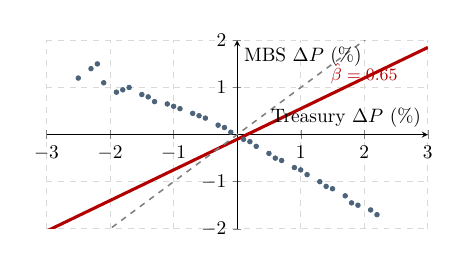
\begin{tikzpicture}[scale=0.7]
  \begin{axis}[
    xlabel={Treasury $\Delta P$ (\%)}, ylabel={MBS $\Delta P$ (\%)},
    xmin=-3, xmax=3, ymin=-2, ymax=2,
    axis lines=middle, width=8.5cm, height=5cm,
    grid=major, grid style={dashed, gray!30}
  ]
  
  \addplot[only marks, mark=*, mark size=1.2pt, navyblue!70] coordinates {
    (-2.5,1.2) (-2.3,1.4) (-2.1,1.1) (-1.9,0.9) (-1.7,1.0) (-1.5,0.85)
    (-1.3,0.7) (-1.1,0.65) (-0.9,0.55) (-0.7,0.45) (-0.5,0.35) (-0.3,0.2)
    (-0.1,0.05) (0.1,-0.1) (0.3,-0.25) (0.5,-0.4) (0.7,-0.55) (0.9,-0.7)
    (1.1,-0.85) (1.3,-1.0) (1.5,-1.15) (1.7,-1.3) (1.9,-1.5) (2.1,-1.6)
    (-2.2,1.5) (-1.8,0.95) (-1.4,0.8) (-1.0,0.6) (-0.6,0.4) (-0.2,0.15)
    (0.2,-0.15) (0.6,-0.5) (1.0,-0.75) (1.4,-1.1) (1.8,-1.45) (2.2,-1.7)
  };
  
  \addplot[domain=-3:3, samples=2, ultra thick, red!70!black] {-0.1 + 0.65*x};
  \addplot[domain=-3:3, samples=2, thick, dashed, gray] {x};
  
  \node[font=\small, red!70!black] at (axis cs:2,1.3) {$\hat{\beta} = 0.65$};
  
  \end{axis}
\end{tikzpicture}
\end{center}

$\hat{\beta} < 1$ reflects MBS negative convexity (smaller gains in rallies).
\end{frame}

\begin{frame}{Principal Component Hedging}
\begin{defbox}[PCA Framework]
Decompose: $\Delta y_t = \sum_{k} \beta_k \cdot PC_{k,t}$ where PC1=level, PC2=slope, PC3=curve.
\end{defbox}

\textbf{Variance Explained:} PC1 $\sim$85\%, PC2 $\sim$10\%, PC3 $\sim$3\%

\begin{center}
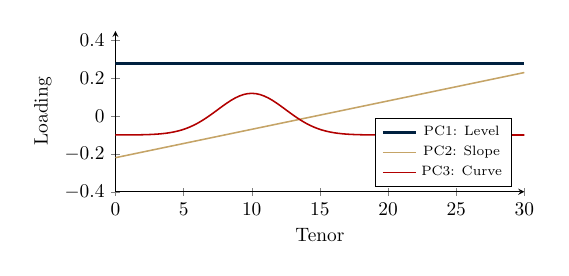
\begin{tikzpicture}[scale=0.7]
  \begin{axis}[
    xlabel={Tenor}, ylabel={Loading},
    xmin=0, xmax=30, ymin=-0.4, ymax=0.45,
    axis lines=left, width=9cm, height=4.5cm,
    legend pos=south east, legend style={font=\scriptsize}
  ]
  
  \addplot[domain=0:30, ultra thick, navyblue] {0.28};
  \addlegendentry{PC1: Level}
  
  \addplot[domain=0:30, thick, goldaccent] {-0.22 + 0.015*x};
  \addlegendentry{PC2: Slope}
  
  \addplot[domain=0:30, samples=100, thick, red!70!black] {0.22*exp(-0.08*(x-10)^2) - 0.1};
  \addlegendentry{PC3: Curve}
  
  \end{axis}
\end{tikzpicture}
\end{center}
\end{frame}

%===============================================
\part{Dynamic Hedging}
\partslide
\section{Rebalancing Framework}
%===============================================

\begin{frame}{Rebalancing: Cost vs.\ Tracking Error}
\begin{defbox}[Rebalancing Trade-off]
\textbf{Tracking Error} (no rebalancing) vs.\ \textbf{Transaction Costs} (frequent rebalancing)
\end{defbox}
\vspace{-0.1cm}
\textbf{Optimal Frequency:} $\boxed{f^* = \sqrt{\frac{\Gamma^2 \sigma_r^4}{4 \cdot TC}}}$ where $TC$ = transaction cost

\begin{center}
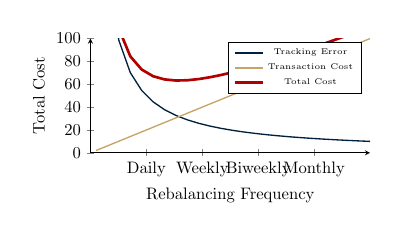
\begin{tikzpicture}[scale=0.6]
  \begin{axis}[
    xlabel={Rebalancing Frequency}, ylabel={Total Cost},
    xmin=0, xmax=50, ymin=0, ymax=100,
    axis lines=left, width=7.5cm, height=4cm,
    xtick={10,20,30,40}, xticklabels={Daily,Weekly,Biweekly,Monthly},
    legend pos=north east, legend style={font=\tiny}
  ]
  
  \addplot[domain=1:50, thick, navyblue] {500/x};
  \addlegendentry{Tracking Error}
  
  \addplot[domain=1:50, thick, goldaccent] {2*x};
  \addlegendentry{Transaction Cost}
  
  \addplot[domain=1:50, ultra thick, red!70!black] {500/x + 2*x};
  \addlegendentry{Total Cost}
  
  \end{axis}
\end{tikzpicture}
\end{center}
\end{frame}

\begin{frame}{Transaction Cost Models}
\begin{defbox}[Cost Components]
\textbf{Total Cost} = Bid-Ask Spread + Market Impact + Opportunity Cost
\end{defbox}
\vspace{-0.1cm}
\textbf{Market Impact (Square-Root):} $\boxed{MI = \sigma \cdot \sqrt{V/ADV} \cdot \text{sign}(V)}$

\textbf{Effective Cost:} $TC_{eff} = \frac{\text{Spread}}{2} + MI + \text{Delay Cost}$

\textbf{Typical Costs:} Treasuries: 0.5-2 bps, Swaps: 0.25-1 bp, TBA: 1-3 bps, Swaptions: 2-10 bps
\end{frame}

\begin{frame}{Gamma Scalping P\&L}
\begin{defbox}[Gamma P\&L]
Daily gamma P\&L: $\boxed{P\&L_\Gamma = \frac{1}{2}\Gamma \cdot (\Delta r)^2 - \Theta \cdot \Delta t}$
\end{defbox}
\vspace{-0.1cm}
\textbf{Expected P\&L:} $\E[P\&L_\Gamma] = \frac{1}{2}\Gamma \cdot \sigma^2 \cdot \Delta t - \Theta \cdot \Delta t$

\textbf{Break-even Volatility:} $\sigma_{BE} = \sqrt{\frac{2\Theta}{\Gamma}}$

\textbf{Interpretation:} If realized vol $>$ implied vol $\Rightarrow$ gamma scalping profitable.
\end{frame}

\begin{frame}{Delta-Gamma-Vega Rebalancing}
\begin{center}
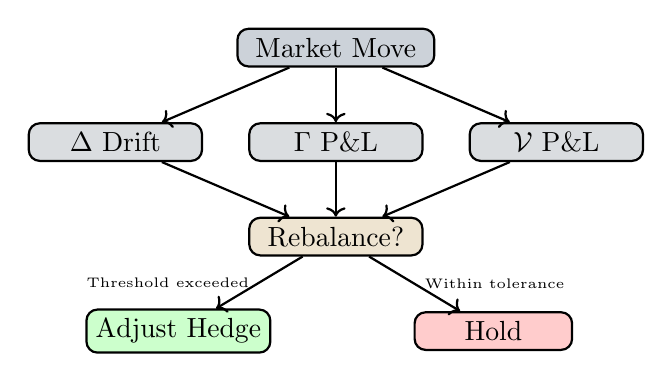
\begin{tikzpicture}[scale=0.8]
  % Flow chart
  \node[draw, thick, fill=navyblue!20, rounded corners, minimum width=2.5cm] (start) at (0,3) {Market Move};
  
  \node[draw, thick, fill=steelgray!20, rounded corners, minimum width=2.2cm] (delta) at (-3.5,1.5) {$\Delta$ Drift};
  \node[draw, thick, fill=steelgray!20, rounded corners, minimum width=2.2cm] (gamma) at (0,1.5) {$\Gamma$ P\&L};
  \node[draw, thick, fill=steelgray!20, rounded corners, minimum width=2.2cm] (vega) at (3.5,1.5) {$\mathcal{V}$ P\&L};
  
  \node[draw, thick, fill=goldaccent!30, rounded corners, minimum width=2.2cm] (rebal) at (0,0) {Rebalance?};
  
  \node[draw, thick, fill=green!20, rounded corners, minimum width=2cm] (yes) at (-2.5,-1.5) {Adjust Hedge};
  \node[draw, thick, fill=red!20, rounded corners, minimum width=2cm] (no) at (2.5,-1.5) {Hold};
  
  \draw[->, thick] (start) -- (delta);
  \draw[->, thick] (start) -- (gamma);
  \draw[->, thick] (start) -- (vega);
  \draw[->, thick] (delta) -- (rebal);
  \draw[->, thick] (gamma) -- (rebal);
  \draw[->, thick] (vega) -- (rebal);
  \draw[->, thick] (rebal) -- node[left, font=\tiny] {Threshold exceeded} (yes);
  \draw[->, thick] (rebal) -- node[right, font=\tiny] {Within tolerance} (no);
\end{tikzpicture}
\end{center}

\textbf{Threshold Rules:} Rebalance when $|\Delta_{actual} - \Delta_{target}| > \epsilon_\Delta$
\end{frame}

%===============================================
\part{Basis \& Spreads}
\partslide
\section{Mortgage Basis}
%===============================================

\begin{frame}{What is Mortgage Basis?}
\begin{defbox}[Basis Definition]
\textbf{Basis} = MBS yield $-$ Benchmark yield

\textbf{Primary Basis} = MBS $-$ Treasury \quad \textbf{Swap Basis} = MBS $-$ Swap
\end{defbox}

\textbf{Basis Components:}
\begin{center}
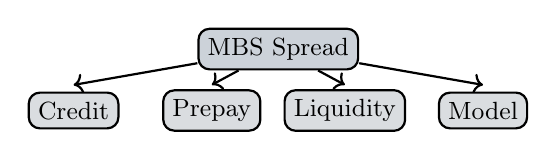
\begin{tikzpicture}[scale=0.65]
  \node[draw, thick, fill=navyblue!20, rounded corners] (basis) at (0,1.2) {\small MBS Spread};
  
  \node[draw, thick, fill=steelgray!20, rounded corners, font=\small] at (-4,0) {Credit};
  \node[draw, thick, fill=steelgray!20, rounded corners, font=\small] at (-1.3,0) {Prepay};
  \node[draw, thick, fill=steelgray!20, rounded corners, font=\small] at (1.3,0) {Liquidity};
  \node[draw, thick, fill=steelgray!20, rounded corners, font=\small] at (4,0) {Model};
  
  \draw[->, thick] (basis) -- (-4,0.5);
  \draw[->, thick] (basis) -- (-1.3,0.5);
  \draw[->, thick] (basis) -- (1.3,0.5);
  \draw[->, thick] (basis) -- (4,0.5);
\end{tikzpicture}
\end{center}

\textbf{Basis P\&L:} $\Delta V_{basis} = -D_{OAS} \cdot P \cdot \Delta OAS$
\end{frame}

\begin{frame}{OAS and Basis Relationship}
\begin{defbox}[Option-Adjusted Spread]
$P_{MBS} = \sum_{paths} \frac{1}{N} \sum_{t} \frac{CF_t^{path}}{(1 + r_t + OAS)^t}$
\end{defbox}

\textbf{Relationship:} Nominal Spread $=$ OAS $+$ Option Cost

\begin{center}
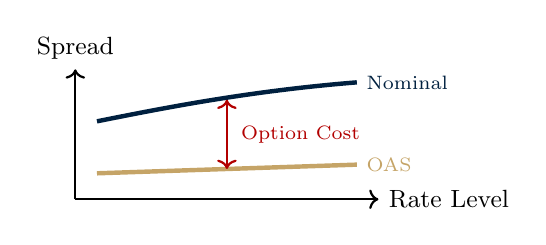
\begin{tikzpicture}[scale=0.55]
  \draw[thick, ->] (0,0) -- (7,0) node[right] {\small Rate Level};
  \draw[thick, ->] (0,0) -- (0,3) node[above] {\small Spread};
  
  \draw[ultra thick, navyblue] (0.5,1.8) .. controls (2,2.1) and (4,2.5) .. (6.5,2.7);
  \node[right, font=\scriptsize, navyblue] at (6.5,2.7) {Nominal};
  
  \draw[ultra thick, goldaccent] (0.5,0.6) -- (6.5,0.8);
  \node[right, font=\scriptsize, goldaccent] at (6.5,0.8) {OAS};
  
  \draw[<->, thick, red!70!black] (3.5,0.7) -- (3.5,2.3);
  \node[right, font=\scriptsize, red!70!black] at (3.6,1.5) {Option Cost};
\end{tikzpicture}
\end{center}
\end{frame}

%===============================================
\section{Advanced Spread Analytics}
%===============================================

\begin{frame}{Z-Spread vs.\ OAS}
\begin{defbox}[Spread Definitions]
\textbf{Z-Spread:} Static spread over spot curve (ignores optionality)
\[
P = \sum_{i=1}^{n} \frac{CF_i}{(1 + s_i + Z)^{t_i}}
\]

\textbf{OAS:} Spread over forward rates after option adjustment
\end{defbox}

\textbf{Relationship:}
\[
\boxed{Z\text{-Spread} \approx OAS + \text{Option Cost}}
\]

\textbf{When to Use:}
\begin{itemize}
  \item Z-Spread: Non-callable bonds, quick relative value
  \item OAS: MBS, callable bonds, comparing across structures
\end{itemize}
\end{frame}

\begin{frame}{LIBOR-OIS and SOFR Basis}
\begin{defbox}[Basis Definitions]
\textbf{LIBOR-OIS Spread:} Credit/liquidity premium in interbank lending

\textbf{SOFR Spread Adjustment:} Transition from LIBOR to SOFR benchmark
\end{defbox}

\textbf{Impact on MBS Hedging:}
\begin{itemize}
  \item Swap hedges reference SOFR (risk-free)
  \item Historical basis risk during LIBOR transition
  \item Spread adjustment $\approx$ 26 bps for 3M LIBOR
\end{itemize}

\textbf{Hedge Adjustment:}
\[
HR_{adj} = HR_{base} \times \left(1 + \frac{\Delta \text{Basis}}{\text{Yield}_{hedge}}\right)
\]
\end{frame}

\begin{frame}{Cross-Currency Basis}
\begin{defbox}[FX Basis]
For non-USD investors, total spread includes FX hedging cost:
\[
\text{Total Spread} = OAS_{MBS} - \text{FX Basis} - \text{Hedge Cost}
\]
\end{defbox}

\textbf{FX Basis Components:}
\begin{itemize}
  \item Forward points (interest rate differential)
  \item Cross-currency basis swap spread
  \item Counterparty credit adjustment
\end{itemize}

\textbf{Example (JPY investor):}
\[
\text{Yield}_{JPY} = \text{Yield}_{USD} - \text{FX Forward Points} - \text{XCCY Basis}
\]
\end{frame}

%===============================================
\part{Empirical Performance}
\partslide
\section{Historical Analysis}
%===============================================

\begin{frame}{Hedge Effectiveness Metrics}
\begin{defbox}[Effectiveness Measures]
\textbf{VRR:} $1 - \frac{\Var(\Delta P_{hedged})}{\Var(\Delta P_{unhedged})}$ \quad \textbf{TE:} $\sqrt{\Var(\Delta P_{MBS} - h \cdot \Delta P_{hedge})}$
\end{defbox}
\vspace{-0.1cm}
\textbf{Typical Hedge Effectiveness:}
\begin{center}
\small
\begin{tabular}{l|c|c}
\toprule
\textbf{Hedge} & \textbf{VRR} & \textbf{TE (bps/mo)} \\
\midrule
Treasuries only & 70-80\% & 15-25 \\
Swaps only & 75-85\% & 12-20 \\
Swaps + Swaptions & 85-92\% & 8-15 \\
TBA + Swaps & 88-95\% & 5-12 \\
\bottomrule
\end{tabular}
\end{center}
\end{frame}

\begin{frame}{Regime-Dependent Hedge Ratios}
\begin{center}
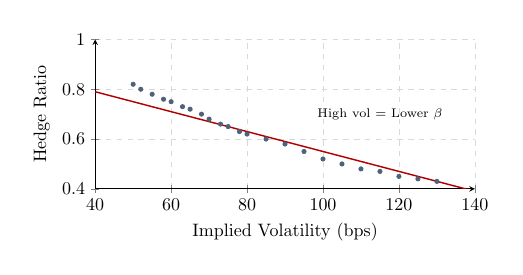
\begin{tikzpicture}[scale=0.65]
  \begin{axis}[
    xlabel={Implied Volatility (bps)}, ylabel={Hedge Ratio},
    xmin=40, xmax=140, ymin=0.4, ymax=1.0,
    axis lines=left, width=9cm, height=4.5cm,
    grid=major, grid style={dashed, gray!30}
  ]
  
  \addplot[only marks, mark=*, mark size=1.2pt, navyblue!70] coordinates {
    (50,0.82) (55,0.78) (60,0.75) (65,0.72) (70,0.68) (75,0.65)
    (80,0.62) (85,0.60) (90,0.58) (95,0.55) (100,0.52) (105,0.50)
    (110,0.48) (115,0.47) (120,0.45) (125,0.44) (130,0.43)
    (52,0.80) (58,0.76) (63,0.73) (68,0.70) (73,0.66) (78,0.63)
  };
  
  \addplot[domain=40:140, thick, red!70!black] {0.95 - 0.004*x};
  
  \node[font=\scriptsize] at (axis cs:115,0.7) {High vol = Lower $\beta$};
  
  \end{axis}
\end{tikzpicture}
\end{center}
\vspace{-0.1cm}
\textbf{Interpretation:} High volatility $\Rightarrow$ MBS underperforms more (negative convexity amplified).
\end{frame}

\begin{frame}{Stress Testing: Rate Shock Scenarios}
\begin{center}
\renewcommand{\arraystretch}{1.2}
\small
\begin{tabular}{l|c|c|c|c}
\toprule
\textbf{Scenario} & \textbf{Rate $\Delta$} & \textbf{MBS} & \textbf{Hedged} & \textbf{Residual} \\
\midrule
\rowcolor{green!10}
Rally 100bp & $-100$ & $+3.5\%$ & $+0.8\%$ & $-2.7\%$ \\
Rally 50bp & $-50$ & $+2.1\%$ & $+0.3\%$ & $-1.8\%$ \\
\rowcolor{navyblue!10}
Unchanged & $0$ & $0\%$ & $0\%$ & $0\%$ \\
Selloff 50bp & $+50$ & $-2.8\%$ & $-0.4\%$ & $+2.4\%$ \\
\rowcolor{red!10}
Selloff 100bp & $+100$ & $-6.2\%$ & $-1.1\%$ & $+5.1\%$ \\
\bottomrule
\end{tabular}
\end{center}

\textbf{Asymmetry:} Hedge performs worse in rally (MBS gains capped) than selloff.
\end{frame}

%===============================================
\section{Historical Case Studies}
%===============================================

\begin{frame}{Case Study: 2013 Taper Tantrum}
\textbf{Event:} Fed signals tapering of QE (May-Aug 2013)

\textbf{Market Impact:}
\begin{itemize}
  \item 10Y Treasury: 1.6\% $\to$ 3.0\% (+140 bps)
  \item MBS OAS: 15 bps $\to$ 45 bps (widened 30 bps)
  \item Implied Vol: 70 $\to$ 110 bps
\end{itemize}

\textbf{Hedge Performance:}
\begin{center}
\small
\begin{tabular}{l|c|c}
\toprule
\textbf{Position} & \textbf{P\&L} & \textbf{Attribution} \\
\midrule
MBS (unhedged) & $-12\%$ & Duration + Convexity + Basis \\
Duration hedge & $+9\%$ & Treasury short \\
\rowcolor{red!10}
Net (duration only) & $-3\%$ & Convexity + Basis \\
\bottomrule
\end{tabular}
\end{center}

\textbf{Lesson:} Duration hedge insufficient; needed convexity + basis protection.
\end{frame}

\begin{frame}{Case Study: 2020 COVID Crisis}
\textbf{Event:} March 2020 liquidity crisis and Fed intervention

\textbf{Market Dynamics:}
\begin{itemize}
  \item Initial: Rates rally, MBS underperforms (negative convexity)
  \item Liquidity crisis: Basis widened 100+ bps
  \item Fed intervention: Purchased \$300B+ MBS
\end{itemize}

\textbf{Key Observations:}
\begin{enumerate}
  \item Correlation breakdown: MBS-Treasury $\rho$ dropped to 0.3
  \item Hedge ratios unstable: Required daily recalibration
  \item Liquidity premium: Transaction costs spiked 5-10x
\end{enumerate}

\textbf{Lesson:} Stress periods require liquidity reserves and pre-positioned hedges.
\end{frame}

\begin{frame}{Case Study: 2022 Rate Hiking Cycle}
\textbf{Event:} Fed raises rates 425 bps (Mar 2022 - Dec 2022)

\textbf{MBS Impact:}
\begin{itemize}
  \item Massive duration extension (prepays collapsed)
  \item Duration increased from 4.5 to 7+ years
  \item Required continuous hedge rebalancing
\end{itemize}

\textbf{Rebalancing Challenge:}
\begin{center}
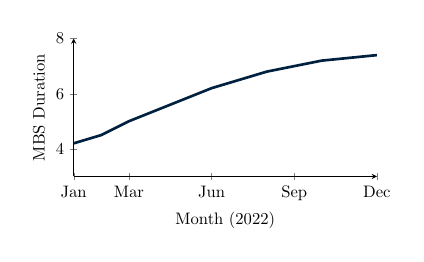
\begin{tikzpicture}[scale=0.6]
  \begin{axis}[
    xlabel={Month (2022)}, ylabel={MBS Duration},
    xmin=1, xmax=12, ymin=3, ymax=8,
    axis lines=left, width=8cm, height=4.5cm,
    xtick={1,3,6,9,12}, xticklabels={Jan,Mar,Jun,Sep,Dec}
  ]
  
  \addplot[ultra thick, navyblue] coordinates {
    (1,4.2) (2,4.5) (3,5.0) (4,5.4) (5,5.8) (6,6.2)
    (7,6.5) (8,6.8) (9,7.0) (10,7.2) (11,7.3) (12,7.4)
  };
  
  \end{axis}
\end{tikzpicture}
\end{center}

\textbf{Lesson:} Hedge ratio must track duration drift; static hedges failed.
\end{frame}

%===============================================
\part{Portfolio \& Risk Management}
\partslide
\section{Portfolio-Level Considerations}
%===============================================

\begin{frame}{Aggregate Portfolio Risk Management}
\begin{defbox}[Portfolio DV01]
\textbf{Aggregate DV01:} $DV01_{portfolio} = \sum_{i} w_i \cdot DV01_i$

\textbf{Aggregate Convexity:} $C_{portfolio} = \sum_{i} w_i \cdot C_i$
\end{defbox}

\textbf{Risk Limits Framework:}
\begin{center}
\small
\begin{tabular}{l|c|c}
\toprule
\textbf{Metric} & \textbf{Limit} & \textbf{Action if Breached} \\
\midrule
Net DV01 & $\pm$\$50K/bp & Rebalance within 24h \\
Net Convexity & $\pm$\$500K/bp$^2$ & Add swaptions \\
OAS Duration & $\pm$1.0 years & Adjust TBA position \\
Vega & $\pm$\$100K/vol pt & Review option book \\
\bottomrule
\end{tabular}
\end{center}
\end{frame}

\begin{frame}{Liability-Driven Hedging (ALM)}
\begin{defbox}[ALM Framework]
For insurers/banks: Hedge \textbf{surplus} = Assets $-$ Liabilities
\[
\Delta S = \Delta A - \Delta L = -D_A \cdot A \cdot \Delta r + D_L \cdot L \cdot \Delta r
\]
\end{defbox}

\textbf{Duration Matching Condition:}
\[
D_A \cdot A = D_L \cdot L \quad \Rightarrow \quad D_A = D_L \cdot \frac{L}{A}
\]

\textbf{Convexity Matching:}
\[
C_A \cdot A = C_L \cdot L
\]

\textbf{Challenge:} MBS negative convexity vs.\ insurance liabilities' positive convexity.
\end{frame}

\begin{frame}{Regulatory Capital Implications}
\begin{defbox}[Basel Treatment]
\textbf{Interest Rate Risk in Banking Book (IRRBB):}

Capital charge based on $\Delta$EVE (Economic Value of Equity) under stress scenarios.
\end{defbox}

\textbf{Hedge Recognition:}
\begin{itemize}
  \item Derivatives must qualify for hedge accounting
  \item Documentation requirements (IAS 39 / ASC 815)
  \item Effectiveness testing: 80-125\% range
\end{itemize}

\textbf{Capital Relief from Hedging:}
\[
\text{Capital}_{hedged} = \text{Capital}_{unhedged} \times (1 - \text{HE})
\]
where HE = hedge effectiveness ratio.
\end{frame}

%===============================================
\section{Numerical Methods}
%===============================================

\begin{frame}{Monte Carlo for Effective Duration}
\begin{defbox}[MC Duration Estimation]
Simulate $N$ interest rate paths, compute:
\[
D_{eff} \approx -\frac{1}{P_0} \cdot \frac{\bar{P}_{-\Delta y} - \bar{P}_{+\Delta y}}{2\Delta y}
\]
where $\bar{P}$ = average price across paths.
\end{defbox}

\textbf{Path Generation (Hull-White):}
\[
dr_t = (\theta(t) - ar_t)dt + \sigma dW_t
\]

\textbf{Convergence:} Standard error $\propto 1/\sqrt{N}$

Typical: $N = 1000-5000$ paths for stable Greeks.
\end{frame}

\begin{frame}{Finite Difference Greeks}
\begin{defbox}[Bump-and-Reprice]
\textbf{Duration:} $D = -\frac{P(y+\Delta y) - P(y-\Delta y)}{2 \cdot P(y) \cdot \Delta y}$

\textbf{Convexity:} $C = \frac{P(y+\Delta y) + P(y-\Delta y) - 2P(y)}{P(y) \cdot (\Delta y)^2}$
\end{defbox}

\textbf{Bump Size Selection:}
\begin{center}
\small
\begin{tabular}{l|c|c}
\toprule
\textbf{Greek} & \textbf{Typical Bump} & \textbf{Issue if Too Small/Large} \\
\midrule
Duration & 10-25 bps & Noise / Non-linearity \\
Convexity & 25-50 bps & Instability / Miss curvature \\
Vega & 1-5 vol pts & Noise / Non-linearity \\
\bottomrule
\end{tabular}
\end{center}

\textbf{Central vs.\ Forward Difference:} Central is more accurate ($O(h^2)$ vs.\ $O(h)$).
\end{frame}

\begin{frame}{Model Risk in Hedging}
\begin{defbox}[Model Risk Sources]
\textbf{Prepayment Model:} Different models $\Rightarrow$ different durations/OAS

\textbf{Interest Rate Model:} Affects option valuation
\end{defbox}

\textbf{Prepayment Model Comparison:}
\begin{center}
\small
\begin{tabular}{l|c|c}
\toprule
\textbf{Model} & \textbf{Duration} & \textbf{OAS} \\
\midrule
Model A (aggressive) & 3.8 yrs & 35 bps \\
Model B (consensus) & 4.2 yrs & 42 bps \\
Model C (conservative) & 4.8 yrs & 55 bps \\
\bottomrule
\end{tabular}
\end{center}

\textbf{Hedge Ratio Range:} Can vary 15-20\% across models!

\textbf{Mitigation:} Use model ensemble, stress test across models.
\end{frame}

%===============================================
\part{Summary}
\partslide
\section{Key Takeaways}
%===============================================

\begin{frame}{Risk Metrics: Master Formulas}
\begin{formulabox}[Core Relationships]
\textbf{Duration Family:}
\[
DV01 = \frac{D_{mod} \times P}{10000} \qquad D_{mod} = -\frac{1}{P}\frac{\pmark P}{\pmark y}
\]

\textbf{Price Change (Full):}
\[
\frac{\Delta P}{P} \approx -D \cdot \Delta y + \frac{1}{2}C \cdot (\Delta y)^2 + \frac{\mathcal{V}}{P} \cdot \Delta\sigma
\]

\textbf{Hedge Ratios:}
\[
h^*_{DV01} = \frac{DV01_{MBS}}{DV01_{hedge}} \qquad h^*_{stat} = \rho \cdot \frac{\sigma_{MBS}}{\sigma_{hedge}}
\]
\end{formulabox}
\end{frame}

\begin{frame}{Hedging Strategy Selection}
\begin{center}
\renewcommand{\arraystretch}{1.15}
\small
\begin{tabular}{l|c|c|c}
\toprule
\textbf{Risk} & \textbf{Instrument} & \textbf{Metric} & \textbf{Cost} \\
\midrule
\rowcolor{navyblue!10}
Duration & Swaps, Futures & DV01 & Low \\
Curve & Multi-tenor swaps & KRD & Low \\
\rowcolor{navyblue!10}
Convexity & Swaptions & Gamma & Medium \\
Volatility & Swaptions & Vega & Medium \\
\rowcolor{navyblue!10}
Basis & TBA, MBS options & OAS Dur & High \\
\bottomrule
\end{tabular}
\end{center}

\textbf{Principles:} (1) Match DV01 first, (2) Add convexity for large portfolios, (3) Use TBA for basis, (4) Rebalance dynamically.
\end{frame}

\begin{frame}{Final Thoughts: The Hedging Trade-off}
\begin{center}
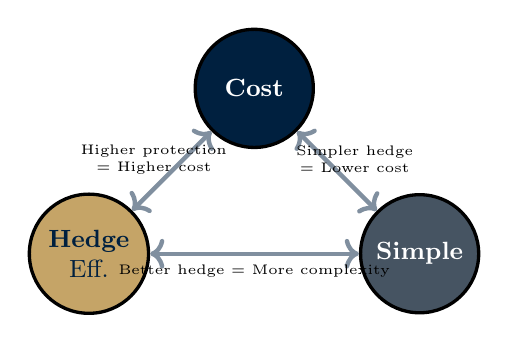
\begin{tikzpicture}[scale=0.75]
  \node[draw, very thick, fill=navyblue, text=white, circle, minimum size=1.5cm, align=center, font=\small] (cost) at (0,2.8) {\textbf{Cost}};
  \node[draw, very thick, fill=goldaccent, text=navyblue, circle, minimum size=1.5cm, align=center, font=\small] (eff) at (-2.8,0) {\textbf{Hedge}\\Eff.};
  \node[draw, very thick, fill=steelgray, text=white, circle, minimum size=1.5cm, align=center, font=\small] (simp) at (2.8,0) {\textbf{Simple}};
  
  \draw[ultra thick, <->, navyblue!50] (cost) -- (eff);
  \draw[ultra thick, <->, navyblue!50] (cost) -- (simp);
  \draw[ultra thick, <->, navyblue!50] (eff) -- (simp);
  
  \node[font=\tiny, align=center] at (-1.7,1.6) {Higher protection\\= Higher cost};
  \node[font=\tiny, align=center] at (1.7,1.6) {Simpler hedge\\= Lower cost};
  \node[font=\tiny, align=center] at (0,-0.3) {Better hedge = More complexity};
\end{tikzpicture}
\end{center}

\textit{Optimal hedging balances protection, cost, and operational feasibility.}
\end{frame}

\begin{frame}
  \vfill
  \centering
  \begin{beamercolorbox}[sep=12pt,center,shadow=true,rounded=true]{palette primary}
    \usebeamerfont{title}\LARGE Questions?\par
  \end{beamercolorbox}
  \vfill
  
  \textbf{References:}
  \begin{itemize}
    \item Fabozzi, F. - \textit{The Handbook of Mortgage-Backed Securities}
    \item Tuckman, B. - \textit{Fixed Income Securities}
    \item Hayre, L. - \textit{Salomon Smith Barney Guide to MBS}
  \end{itemize}
\end{frame}

\end{document}